\section{Formal verification in presence of unbounded loops\label{sec-motor-control}}

In the last section we have demonstrated the framework's capabilities for
formal verification on an example of the energy estimation program.
Many programs targeting REDFIN share the distinctive feature of
this example and have statically predictable upper \emph{bound on execution time}
thanks to the fact that their termination does not
depend on the input data. However, some control programs may have loops
which are guarded by termination conditions that involve computation
considering the input parameters of the program, thus making the loop
\emph{unbounded}.

The presence of unbounded loops makes whole-program
verification inapplicable in the general case~\cite{some-paper-on-symexec},
since the state space of the program becomes huge or even infinite. However,
if the program essentially comprises a single unbounded loop, some properties
of the program could be verified by determining the \emph{loop invariant}
and proving that it holds for every iteration of the loop.

In this section we apply the developed verification framework to a larger
example of a stepper motor control program and make an accent on how
the presence of an unbounded loop may be mitigated and which properties
of the program can be verified with symbolic execution.

\subsection{Stepper motor control program}

Stepper motors are often deployed as parts of antenna and solar panel pointing units
in space satellites. We consider a control program for controlling a motor with
one degree of freedom. The program, given the distance to move the motor and safety
bounds on velocity and acceleration, will compute a series of speed and velocity values
that can be used to move the motor.

The algorithm~\ref{alg-motor} expects three input
parameters: $dist$ --- the distance to move the motor, $v\_max$ --- the maximal permitted
velocity and $a\_max$ --- the maximal permitted acceleration. The conditional statement on
line 9 decided whether to accelerate the motor, to keep it on steady speed or to decelerate
it; see~\ref{fig-motor} for plots of velocity and distance travelled against time. The
spike on the bottom-left of the velocity graph illustrates the edge case when the $dist$
parameter is not divisible by $a\_max$ (\todo{check this bit}).

\begin{algorithm}[h]
  \label{alg-motor}
  \begin{algorithmic}[1]
\Require {$dist$, $v\_max$, $a\_max$}
\State $s \gets 0$
\State $v \gets 0$
\While {$true$}
  % Compute deceleration distance based on current speed
  \State $decel\_steps\gets \lfloor v / a\_max \rfloor$
  \algorithmiccomment{# Compute deceleration distance based on current speed}
  \State $s\_decel \gets a\_max \cdot (decel\_steps + 1) / 2$
  \If {$decel\_steps \cdot a\_max \neq v$}
    \State $s\_decel \gets s\_decel + v$
  \EndIf
  \State {$v\_next = min(v\_max, dist, v + a\_max)$}
  \If {$s + s\_decel + v\_next \leq dist$}
    \State $v \gets v\_next$ \algorithmiccomment{accelerate}
  \ElsIf {$s + s\_decel + v \leq dist$}
    \State $ v \gets v $     \algorithmiccomment{keep speed}
  \Else
     \algorithmiccomment{decelerate}
    \If {$v > decel\_steps \cdot a\_max$}
      \State $v \gets decel\_steps \cdot a\_max$
    \Else
      \State $v \gets v - a\_max$
    \EndIf
  \If {$v = 0$}
    \If {$s \neq dist$}  \algorithmiccomment{accelerate again to reach target}
      % didn't quite reach our target after deceleration
      % => accelerate again
      \State $v \gets min(dist - s, a\_max)$
    \Else
      % reached target
      \State $break$  \algorithmiccomment{terminate execution}
  \EndIf
\EndWhile
\end{algorithmic}
\caption{Motor Control Algorithm}
\end{algorithm}

\begin{figure}[h]
\centerline{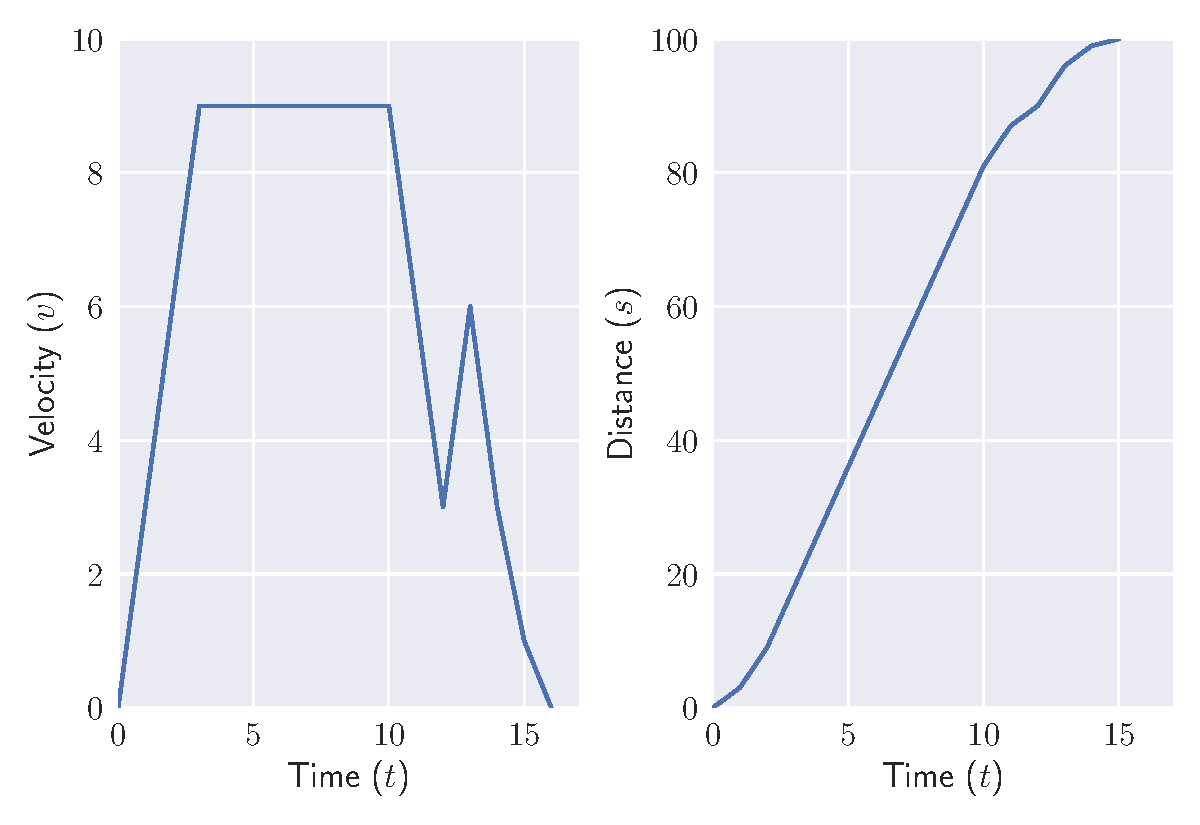
\includegraphics[scale=0.6]{fig/motor_control_graph.pdf}}
\caption{Motor control program execution\label{fig-motor}}
\Description[Please consult the text of this section for the description]{}
\end{figure}

To be deployed into Redfin, the algorithm~\ref{alg-motor} must be manually
re-implemented in Redfin assembly. The resulting assembly program comprises 85 lines of
code and mostly mirrors the pseudocode of the algorithm.

\subsection{Loop invariant verification}

In order to ensure that the motor will not introduce disturbances
and will not lead the whole unit out of its normal mode of operation, the velocity and
acceleration of the motor must be kept in safe limits. More formally, that would mean
that in any iteration of the loop the values of the expressions $v$, the velocity,
and $\left| v\_next - v \right|$, the acceleration, never exceed the
parameters $v\_max$ and $a\_max$,
respectively. This property is the loop invariant for the motor control program which
ensures that velocity and acceleration always stay within their safe bounds. We can
formalise it as the following predicate that quantifies over the program's inputs and
state:

\begin{figure}[h]
\[
  \forall\ v\_max\ a\_max\ v\ v\_next\ s,
  \ v\ \leq v\_max\ \land\ \left| v\_next - v \right| \leq a\_max
\]
\caption{Loop invariant: velocity and acceleration are within bounds}
\end{figure}

We will verify the loop invariant by using the verification framework in the
\emph{branching mode}\ref{sec-operation-modes}. While symbolic execution with
merging, which is implemented by the framework's \emph{mergin} mode, allows
for intuitive formulation of properties for whole-program verification and
is very useful for finite programs and programs with bounded loops, as we have
reported in the previous sections, in presence of branches that depended on
symbolic values it suppers from \emph{symbolic termination}. Thus, for verifying the
loop invariant, we rely on traditional symbolic execution.

To verify the loop invariant we take the following approach:

\begin{itemize}
  \item Obtain the binary tree-shaped trace by \emph{bounded} symbolic execution
  in \emph{branching} mode
  \item Split the trace into linear paths, thus enumerating all the possible
    execution scenarios
  \item For every path perform the analysis
    \begin{enumerate}
      \item Extract the relevant parts of the state from the \emph{last} node in
            the path, i.e. symbolic expressions stored in
            registers, memory cells or flags
      \item Construct a symbolic expression representing the \emph{property to check},
            which would involve the expressions obtained in the previous step
      \item Extract the \emph{path condition} from the /last/ node in the path
      \item Formulate the \emph{preconditions} of the program
      \item To verify the property in the given path by checking the following
            formula for satisfiability:
              preconditions /\ path constraints /\ ¬ property to check
    \end{enumerate}
    \item  The property holds if and only if for every path the solver returns
           \hs{Unsatisfiable}, i.e. there are no assignments of the variables which
           satisfy the~\emph{negation} of the property to check, considering the
           preconditions and the path condition.
\end{itemize}

This detailed verification algorithms has several parameters that need to be specified:

\begin{itemize}
\item Preconditions on $v\_max$ and $a\_max$
\item Symbolic execution bound, i.e. for how many steps perform the execution. Since the
      body of the loop will always terminate this bound can be calculated in advance.
\end{itemize}

\subsection{Pruning branches}

Every conditional jump instruction produces two branches in the execution tree: the one
where the path condition is conjoined with the jump's guard and the one where it is
conjoined with the guard's negation~\ref{fig-sym-tree}. However, if the resulting
conjunction is unsatisfiable, the corresponding branch does not have to be explored
and can be pruned. Thus the symbolic execution engine need to call an SMT solver every
time a conditional jump is encountered to check if the path conditions of the branches
are satisfiable.

Checking satisfiability of execution path is essential to mitigation the path explosion
problem. Pre-condition, when available, is assigned as the initial path condition and thus
will become a subterm of every formula submitted to the solver. Identifying correct pre-conditions is essential for verification since they may drastically reduce the number of satisfiable paths in the symbolic execution tree of the program that is being verified.

\begin{figure}[h]
\centerline{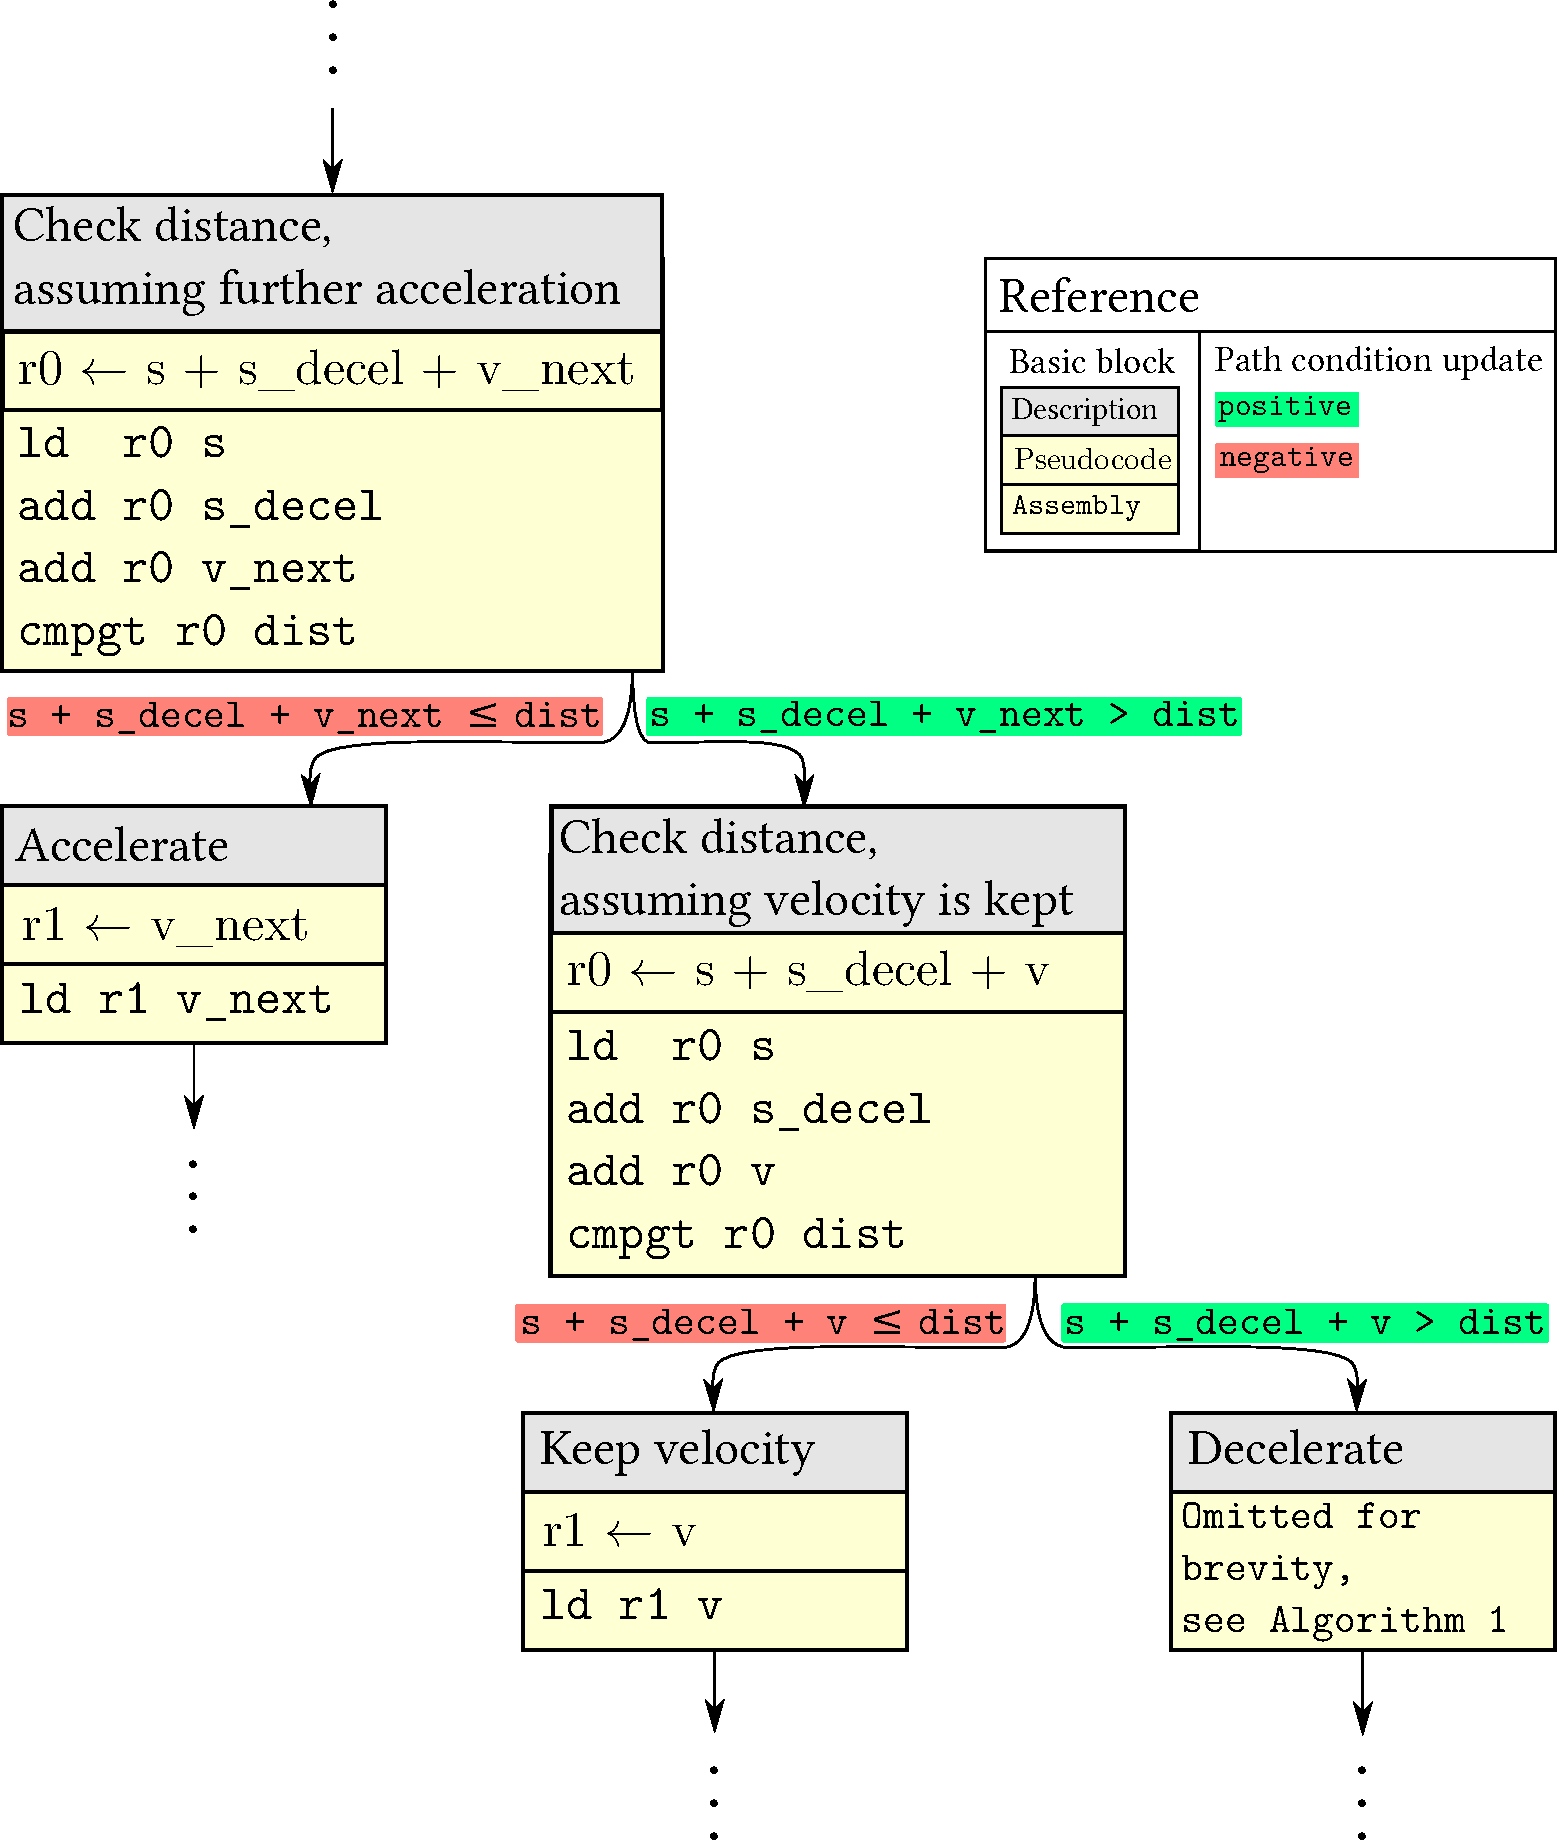
\includegraphics[scale=0.4]{fig/sym-tree.pdf}}
\caption{Branching symbolic execution\label{fig-sym-tree}}
\Description[Please consult the text of this section for the description]{}
\caption{Loop invariant: velocity and acceleration are within bounds}
\end{figure}



Give the preconditions, an example of the execution path, talk about constant folding
and SMT-solving to prove unsatisfiable paths, make a table(?) with results for different
preconditions: number of path, time to solve a path, length of the path maybe.

\subsection{NOTES}

``Pre-conditions, when
available, may be leveraged to reduce the size of the input
data domains and to only generate test inputs that satisfy
the pre-conditions.''


---
